\section{Accessibilità}
	\subsection{Separazione tra contenuto, presentazione e struttura}
	\par Per migliorare la qualità dell’utilizzo del sito agli utenti con disabilità  è stato posto l’accento sulla separazione tra presentazione, struttura e comportamento.
La separazione è stata implementata tramite documenti XHTML strict 1.0, che richiamano fogli di stile CSS esterni.
	\par Nonostante il controllo input e i messaggi di errore siano stati realizzati in JavaScript, esistono funzioni PHP per le stesse operazioni che permettono il corretto funzionamento del sito anche su dispositivi che non lo supportano.
La totalità del codice è stata scritta seguendo le raccomandazioni del \textbf{W3C}\footnote{\url{https://www.w3.org/}}, accertandosi che fossero rispettate tramite validazione.
	\subsection{Facilitazioni per la navigazione}
	\par L’interfaccia del sito è stata ideata per avere una navigazione comoda attraverso tab, non è stato quindi necessario aggiungere un attributo \texttt{tabindex} per dare un ordine prioritario alle tabulazioni. Tutte le immagini sono state marcate con apposite label e tag \texttt{alt}.
	\par In modo da poter essere accessibile da dispositivi con schermi di dimensioni minori rispetto ai desktop, il sito web è stato costruito per avere un layout \textit{responsive}. Sempre con questo scopo è stata posta particolare attenzione allo sviluppo orizzontale del sito, evitando in qualunque circostanza lo scroll orizzontale. Questo è risultato fondamentale per l’usabilità del sito su smartphone.
	\par Con lo scopo di minimizzare il disorientamento e la confusione dei visitatori è stata creata una pagina di \textbf{errore 404}, contenente link utili a riprendere la navigazione nel sito e un logo personalizzato che, oltre ad aggiungere particolarità alla pagina, cerca di ridurre la frustrazione dell’utente sfruttando l’ironia.
	\par Ogni link è stato reso distinguibile da ogni altro tramite apposite regole di stile, \textbf{hover} e \textbf{visited}: nel caso dell’hover la sottolineatura del link si ispessisce e scurisce, nel caso del visited il link cambia colore. All’apice di ogni pagina è presente una barra di navigazione composta da collegamenti rapidi alle funzionalit\`a pi\`u importanti del sito. Ogni qualvolta l’utente si trovi in una pagina corrispondente ad una di queste funzionalit\`a il relativo collegamento si evidenzia in modo aiutare l'utente nell'orientamento. Inoltre, avendo rispettato la regola dei 4 click, non abbiamo giudicato necessaria la creazione di una sitemap.
	\par Un ulteriore aiuto al visitatore viene fornito dal breadcrumb. Il breadcrumb \`e una lista ordinata di collegamenti ipertestuali alle pagine che rappresentano il percorso dalla pagina iniziale alla pagina corrente. Ogni elemento della lista \`e separato da un front slash e l’ultimo elemento, che è la pagina corrente, non ha link. Esso consente di tornare con facilità alle pagine visitate in precedenza.
	\par L’accessibilità del sito è stata migliorata ulteriormente dalla presenza di un tasto ancora che permette di tornare all’apice della pagina.
  \par Tutte parole di lingua diversa da quella italiana sono state racchiuse all’interno di tag con l’attributo lang, per permettere una corretta lettura da parte degli screen reader.
	\subsection{Schema colori}
	\par Per quello che concerne l’accessibilità delle categorie di utenti con difficoltà visive si è deciso di usare unicamente colori \quotes{\textbf{web safe}}, mantenendo sempre un contrasto elevato tra lo sfondo e le scritte, evitando così di renderle meno leggibili; non è presente inoltre alcun contenuto pericoloso per utenti a rischio epilessia, o contenuti che possano indurre l’utente in stato confusionale. 
Per quanto riguarda le immagini non è stato possibile fare molto perché vengono caricate da utenti, è possibile però ingrandirle cliccandoci sopra.
	\par(Inserire screenshot del sito versione desktop anche con modalità per disabili)
	\begin{figure}[!htb]
		\center{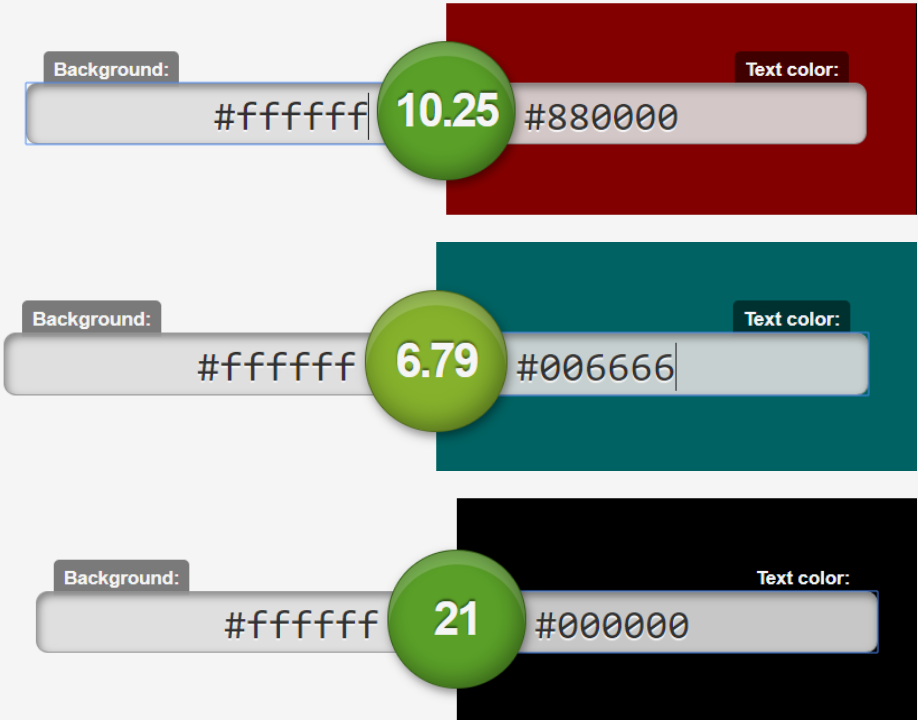
\includegraphics[width=\textwidth]{colors}}
		\caption{\label{fig:ganttAnalisi} Schema dei colori}
	\end{figure}
	\subsection{Accessibilità mobile}
	\par L’accessibilità per mobile è stata sviluppata con CSS puro, questo ha garantito la compatibilità con la maggior parte dei dispositivi mobile.
	\par(Inserire screenshot del sito versione mobile)
	\subsection{CSS di stampa}
  \par Viene incluso un layout di stampa per ogni pagina: le informazioni principali di una pagina vengono estrapolate e organizzate in un formato adeguato. Sono stati tolti tutti gli elementi visivi non strettamente necessari al contenuto, quindi tutte le immagini di background o di presentazione. Abbiamo rimosso anche il menu, la barra di ricerca, il footer e tutti i form di ricerca e di invio di un messaggio perch\'e non ne abbiamo ritenuta fondamentale la visualizzazione su una pagina stampata. Tuttavia abbiamo deciso di mantere il form per la creazione e modifica di un annuncio perch\'e, essendoci molti campi da compilare per le caratteristiche di un'autovettura, all'utente pu\`o tornare utile avere traccia di quali informazioni sono richieste per completare un'annuncio.
  
  \par (Inserire screenshot)
	

